An op amp with open-loop voltage gain of $10^{4}$ and poles at $10^{6},10^{7} $and$ 10^{8}$ Hz is to be compensated by the addition of a fourth dominant pole to operate stably with unity feedback ($|H| = 1$). What is the frequency of the required dominant pole? The compensation network placed in the negative feedback path of the op amp. The dc bias conditions are such that a $1M\Omega$ resistor can be tolerated in series with each of the negative and positive input terminals. What capacitor is required between the negative input and ground to implement the required fourth pole?
\begin{enumerate}[label=\arabic*.,ref=\theenumi]
%\begin{enumerate}[label=\thesection.\arabic*.,ref=\thesection.\theenumi]
\numberwithin{equation}{enumi}

\item Find $G(s)$ for the OPAMP.
%\renewcommand{\thefigure}{\theenumi.\arabic{figure}}
\\
\solution
\begin{align}
G(s) = \frac{G_0}{\brak{1+\frac{s}{P_{1}}}\brak{1+\frac{s}{P_{2}}}\brak{1+\frac{s}{P_{3}}}}
\end{align}
%
where the gain and poles are listd in Table \ref{table:ee18btech11026_Table_1}.
%
\begin{table}[!ht]
\centering


%%  This section checks if we are begin input into another file or  %%
%%  the file will be compiled alone. First use a macro taken from   %%
%%  the TeXbook ex 7.7 (suggestion of Han-Wen Nienhuys).            %%
\def\ifundefined#1{\expandafter\ifx\csname#1\endcsname\relax}


%%  Check for the \def token for inputed files. If it is not        %%
%%  defined, the file will be processed as a standalone and the     %%
%%  preamble will be used.                                          %%
\ifundefined{inputGnumericTable}

%%  We must be able to close or not the document at the end.        %%
	\def\gnumericTableEnd{\end{document}}


%%%%%%%%%%%%%%%%%%%%%%%%%%%%%%%%%%%%%%%%%%%%%%%%%%%%%%%%%%%%%%%%%%%%%%
%%                                                                  %%
%%  This is the PREAMBLE. Change these values to get the right      %%
%%  paper size and other niceties.                                  %%
%%                                                                  %%
%%%%%%%%%%%%%%%%%%%%%%%%%%%%%%%%%%%%%%%%%%%%%%%%%%%%%%%%%%%%%%%%%%%%%%

	\documentclass[12pt%
			  %,landscape%
                    ]{report}
       \usepackage[latin1]{inputenc}
       \usepackage{fullpage}
       \usepackage{color}
       \usepackage{array}
       \usepackage{longtable}
       \usepackage{calc}
       \usepackage{multirow}
       \usepackage{hhline}
       \usepackage{ifthen}
%%  End of the preamble for the standalone. The next section is for %%
%%  documents which are included into other LaTeX2e files.          %%
\else

%%  We are not a stand alone document. For a regular table, we will %%
%%  have no preamble and only define the closing to mean nothing.   %%
    \def\gnumericTableEnd{}

%%  If we want landscape mode in an embedded document, comment out  %%
%%  the line above and uncomment the two below. The table will      %%
%%  begin on a new page and run in landscape mode.                  %%
%       \def\gnumericTableEnd{\end{landscape}}
%       \begin{landscape}


%%  End of the else clause for this file being \input.              %%
\fi

%%%%%%%%%%%%%%%%%%%%%%%%%%%%%%%%%%%%%%%%%%%%%%%%%%%%%%%%%%%%%%%%%%%%%%
%%                                                                  %%
%%  The rest is the gnumeric table, except for the closing          %%
%%  statement. Changes below will alter the table's appearance.     %%
%%                                                                  %%
%%%%%%%%%%%%%%%%%%%%%%%%%%%%%%%%%%%%%%%%%%%%%%%%%%%%%%%%%%%%%%%%%%%%%%

\providecommand{\gnumericmathit}[1]{#1} 
%%  Uncomment the next line if you would like your numbers to be in %%
%%  italics if they are italizised in the gnumeric table.           %%
%\renewcommand{\gnumericmathit}[1]{\mathit{#1}}
\providecommand{\gnumericPB}[1]%
{\let\gnumericTemp=\\#1\let\\=\gnumericTemp\hspace{0pt}}
 \ifundefined{gnumericTableWidthDefined}
        \newlength{\gnumericTableWidth}
        \newlength{\gnumericTableWidthComplete}
        \newlength{\gnumericMultiRowLength}
        \global\def\gnumericTableWidthDefined{}
 \fi
%% The following setting protects this code from babel shorthands.  %%
 \ifthenelse{\isundefined{\languageshorthands}}{}{\languageshorthands{english}}
%%  The default table format retains the relative column widths of  %%
%%  gnumeric. They can easily be changed to c, r or l. In that case %%
%%  you may want to comment out the next line and uncomment the one %%
%%  thereafter                                                      %%
\providecommand\gnumbox{\makebox[0pt]}
%%\providecommand\gnumbox[1][]{\makebox}

%% to adjust positions in multirow situations                       %%
\setlength{\bigstrutjot}{\jot}
\setlength{\extrarowheight}{\doublerulesep}

%%  The \setlongtables command keeps column widths the same across  %%
%%  pages. Simply comment out next line for varying column widths.  %%
\setlongtables

\setlength\gnumericTableWidth{%
	60pt+%
	100pt+%
0pt}
\def\gumericNumCols{2}
\setlength\gnumericTableWidthComplete{\gnumericTableWidth+%
         \tabcolsep*\gumericNumCols*2+\arrayrulewidth*\gumericNumCols}
\ifthenelse{\lengthtest{\gnumericTableWidthComplete > \linewidth}}%
         {\def\gnumericScale{\ratio{\linewidth-%
                        \tabcolsep*\gumericNumCols*2-%
                        \arrayrulewidth*\gumericNumCols}%
{\gnumericTableWidth}}}%
{\def\gnumericScale{1}}

%%%%%%%%%%%%%%%%%%%%%%%%%%%%%%%%%%%%%%%%%%%%%%%%%%%%%%%%%%%%%%%%%%%%%%
%%                                                                  %%
%% The following are the widths of the various columns. We are      %%
%% defining them here because then they are easier to change.       %%
%% Depending on the cell formats we may use them more than once.    %%
%%                                                                  %%
%%%%%%%%%%%%%%%%%%%%%%%%%%%%%%%%%%%%%%%%%%%%%%%%%%%%%%%%%%%%%%%%%%%%%%

\ifthenelse{\isundefined{\gnumericColA}}{\newlength{\gnumericColA}}{}\settowidth{\gnumericColA}{\begin{tabular}{@{}p{60pt*\gnumericScale}@{}}x\end{tabular}}
\ifthenelse{\isundefined{\gnumericColB}}{\newlength{\gnumericColB}}{}\settowidth{\gnumericColB}{\begin{tabular}{@{}p{100pt*\gnumericScale}@{}}x\end{tabular}}
\begin{tabular}[c]{%
	b{\gnumericColA}%
	b{\gnumericColB}%%
	}

%%%%%%%%%%%%%%%%%%%%%%%%%%%%%%%%%%%%%%%%%%%%%%%%%%%%%%%%%%%%%%%%%%%%%%
%%  The longtable options. (Caption, headers... see Goosens, p.124) %%
%	\caption{The Table Caption.}             \\	%
% \hline	% Across the top of the table.
%%  The rest of these options are table rows which are placed on    %%
%%  the first, last or every page. Use \multicolumn if you want.    %%

%%  Header for the first page.                                      %%
%	\multicolumn{3}{c}{The First Header} \\ \hline 
%	\multicolumn{1}{c}{colTag}	%Column 1
%	&\multicolumn{1}{c}{colTag}	%Column 2
%	&\multicolumn{1}{c}{colTag}	\\ \hline %Last column
%	\endfirsthead

%%  The running header definition.                                  %%
%	\hline
%	\multicolumn{3}{l}{\ldots\small\slshape continued} \\ \hline
%	\multicolumn{1}{c}{colTag}	%Column 1
%	&\multicolumn{1}{c}{colTag}	%Column 2
%	&\multicolumn{1}{c}{colTag}	\\ \hline %Last column
%	\endhead

%%  The running footer definition.                                  %%
%	\hline
%	\multicolumn{3}{r}{\small\slshape continued\ldots} \\
%	\endfoot

%%  The ending footer definition.                                   %%
%	\multicolumn{3}{c}{That's all folks} \\ \hline 
%	\endlastfoot
%%%%%%%%%%%%%%%%%%%%%%%%%%%%%%%%%%%%%%%%%%%%%%%%%%%%%%%%%%%%%%%%%%%%%%

\hhline{|-|-}
	 \multicolumn{1}{|p{\gnumericColA}|}%
	{\gnumericPB{\centering}\textbf{Parameters}}
	&\multicolumn{1}{p{\gnumericColB}|}%
	{\gnumericPB{\centering}\textbf{Value}}

	
\\


\hhline{|--|}
	 \multicolumn{1}{|p{\gnumericColA}|}%
	{\gnumericPB{\centering}$P_{1}$}
	&\multicolumn{1}{p{\gnumericColB}|}%
	{\gnumericPB{\centering}$2\pi  10^{6}$ rad/sec}


\\


\hhline{|--|}
	 \multicolumn{1}{|p{\gnumericColA}|}%
	{\gnumericPB{\centering}$P_{2}$}
	&\multicolumn{1}{p{\gnumericColB}|}%
	{\gnumericPB{\centering}$2\pi  10^{7}$ rad/sec}


\\

\hhline{|--|}
	 \multicolumn{1}{|p{\gnumericColA}|}%
	{\gnumericPB{\centering}$P_{3}$}
	&\multicolumn{1}{p{\gnumericColB}|}%
	{\gnumericPB{\centering}$2\pi  10^{8}$ rad/sec}


\\



\hhline{|--|}
	 \multicolumn{1}{|p{\gnumericColA}|}%
	{\gnumericPB{\centering}$G_0$}
	&\multicolumn{1}{p{\gnumericColB}|}%
	{\gnumericPB{\centering}$10^{4}$}



\\
\hhline{|-|-|}
\end{tabular}

\ifthenelse{\isundefined{\languageshorthands}}{}{\languageshorthands{\languagename}}
\gnumericTableEnd


\caption{}
\label{table:ee18btech11026_Table_1}
\end{table}
%
%\item Examine the stability of the feedback system with open loop gain $G(s)$ and feedback $H=1$.
%\\
%\solution Find the poles of $T(s)$
\item Find the 4th dominant pole $P_D$ that will stabilize the system.
\\
\solution Let the pole frequency be $f_D$.  The 4 pole system will be stable if 
 the gain begins to rolloff from 80dB at a -20 dB/dec rate  from $f_{D}$ and continues  until $f_{P1}$ where it cuts 0dB line. From Fig. \ref{fig:ee18btech11026_1}, 
\begin{align}
f_{D} &= \frac{f_{P1}}{10^{4}}\\
\implies f_{D} &= 10^{2} Hz
\end{align}  

\begin{figure}[!h]
    \centering
    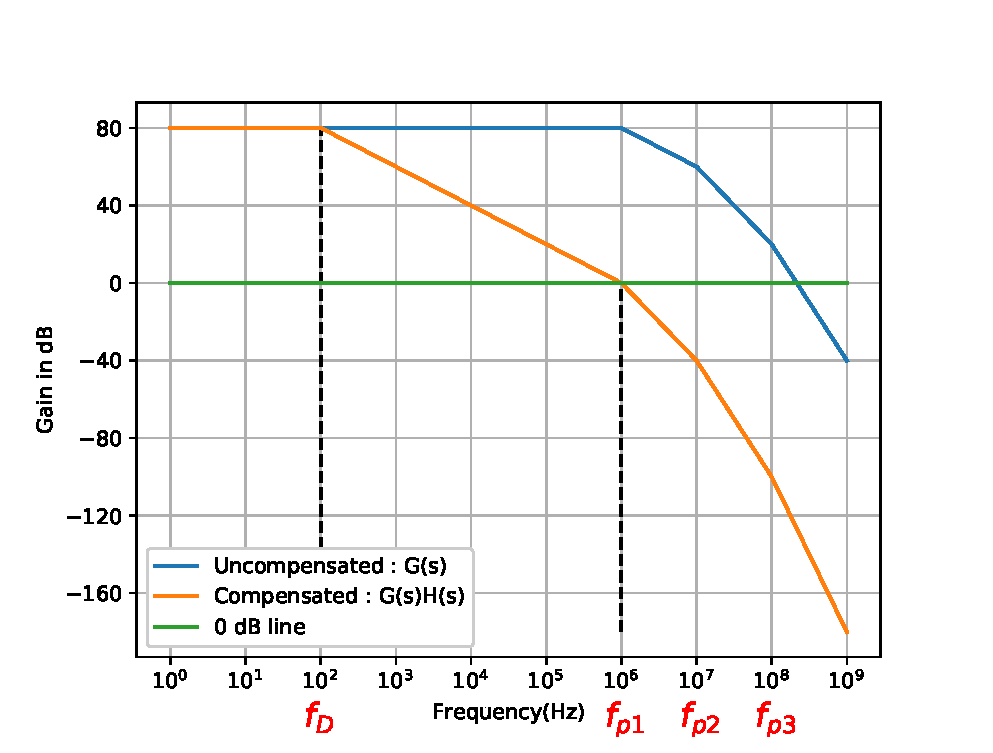
\includegraphics[width=\columnwidth]{./figs/ee18btech11026/ee18btech11026_1.eps}
    \caption{Bode Plot using asymptotic approximations}
    \label{fig:ee18btech11026_1}
\end{figure}
\item Draw the block diagram for the stabilized circuit.
\\
\solution See Fig. \ref{fig:ee18btech110026_block}, where 
\begin{align}
P_D = \frac{1}{R_fC_f}
\end{align}

\begin{figure}[!ht]
	\begin{center}
				\resizebox{\columnwidth}{!}{\tikzstyle{block} = [draw, rectangle, 
    minimum height=1.25em, minimum width=2.5em]
\tikzstyle{sum} = [draw, circle, node distance=1cm]
\tikzstyle{input} = [coordinate]
\tikzstyle{output} = [coordinate]
\tikzstyle{pinstyle} = [pin edge={to-,thin,black}]

% The block diagram code is probably more verbose than necessary
\begin{tikzpicture}[auto, node distance=2.5cm,>=latex']
    % We start by placing the blocks
    \node [input, name=input] {};
    \node [sum, right of=input] (sum) {};
    \node [block, right of=sum] (controller) {$\frac{10^{4}}{\brak{1+\frac{s}{P_{1}}}\brak{1+\frac{s}{P_{2}}}\brak{1+\frac{s}{P_{3}}}}$};
    
    % We draw an edge between the controller and system block to 
    % calculate the coordinate u. We need it to place the measurement block. 
   
    \node [output, right of=controller] (output) {};
    \node [block, below of=controller] (measurements) {$\frac{1}{1+sR_{f}C_{f}}$};

    % Once the nodes are placed, connecting them is easy. 
    \draw [draw,->] (input) -- node[pos=0.99] {$+$} node {$V_{s}$} (sum);
    \draw [->] (sum) -- node {$V_{i}$} (controller);
    \draw [->] (controller) -- node [name=y] {$V_{o}$}(output);
    \draw [->] (y) |- (measurements);
    \draw [->] (measurements) -| node[pos=0.99] {$-$} node [near end] {$V_{f}$} (sum);
\end{tikzpicture}
}
	\end{center}
\caption{Block Diagram}
\label{fig:ee18btech110026_block}
\end{figure}
%
\item Design the OPAMP circuit for Fig. \ref{fig:ee18btech110026_block}.
\\
\solution See Fig. \ref{fig:ee18btech110026_circuit_1}.
\begin{align}
H(s) = \frac{V_{f}}{V_{0}}
	&= \frac{1}{1+sR_{f}C_{f}}
\end{align}

%
\begin{figure}[!ht]
	\begin{center}
				\resizebox{\columnwidth}{!}{\begin{circuitikz}
\ctikzset{bipoles/length=1cm}

\draw 
(0, 0) node[op amp] (opamp) {}
(opamp.-) -- (-2.5,0.35) to[C,l_=$C_{f}$,*-*] (-3.5, 0.35) to (-4, 0.35) to (-4.5, 0.35) node[ground]{}
(opamp.-) --(-0.85,1) to[R=$R_{f}$] (1,1) -- (1,0) --(2,0) node at(2.3,0){$V_0$}
(opamp.out) to (1,0)%--(1.5,-0.5)% to[R=$R_L$] (1.5,-1.5) to (1.5,-1.5) node[ground]{}
(opamp.+) -- (-0.6,-0.35) to[R =$R_s$,*-*] (-2.6,-0.35) to[V=$V_s$] (-2.6,-2.4) node[ground]{}
node at(-3.5,0.1){$-$}
node at(-2.5,0.1){$+$}
node at(-3,-0.3){$V_f$}
node at (-0.1,0){$G(s)$}
;\end{circuitikz}

}
	\end{center}
\caption{}
\label{fig:ee18btech110026_circuit_1}
\end{figure}
%
%For $P_{D}$ to become a dominant pole, $f_D < f_1$.
%Also, $f_{D}$ should be such that the modified loop gain intersects the $20log(\frac{1}{|H(s)|})$ with -20 dB slope  near $f_{P1}$ , so as to ensure stability. 
%\\
%Since its unity feedback , the loop gain should intersect the 0dB line at $f_{P1}$\\
%\\As shown in Fig:\ref{fig:ee18btech11026_1}:
%
%This extra pole is achieved through a Low-pass series RC network placed in the negative feedback as shown in the figure \ref{fig:ee18btech110026_circuit_1}.

\item Find $R_f$ and $C_f$.
\\
\solution
\begin{align}
\because P_{D} &=2\pi  f_{D},
\\
C_{f} &= \frac{1}{2\pi R_{f}f_{D}}
\end{align}
%
Choosing
\begin{align}
R_{f} = R_{s}=1M\Omega,
 C_{f} &= 1.59nF
\end{align}
%
Table \ref{table:ee18btech11026_Table_2} summarizes this.
%
\begin{table}[!ht]
\centering


%%  This section checks if we are begin input into another file or  %%
%%  the file will be compiled alone. First use a macro taken from   %%
%%  the TeXbook ex 7.7 (suggestion of Han-Wen Nienhuys).            %%
\def\ifundefined#1{\expandafter\ifx\csname#1\endcsname\relax}


%%  Check for the \def token for inputed files. If it is not        %%
%%  defined, the file will be processed as a standalone and the     %%
%%  preamble will be used.                                          %%
\ifundefined{inputGnumericTable}

%%  We must be able to close or not the document at the end.        %%
	\def\gnumericTableEnd{\end{document}}


%%%%%%%%%%%%%%%%%%%%%%%%%%%%%%%%%%%%%%%%%%%%%%%%%%%%%%%%%%%%%%%%%%%%%%
%%                                                                  %%
%%  This is the PREAMBLE. Change these values to get the right      %%
%%  paper size and other niceties.                                  %%
%%                                                                  %%
%%%%%%%%%%%%%%%%%%%%%%%%%%%%%%%%%%%%%%%%%%%%%%%%%%%%%%%%%%%%%%%%%%%%%%

	\documentclass[12pt%
			  %,landscape%
                    ]{report}
       \usepackage[latin1]{inputenc}
       \usepackage{fullpage}
       \usepackage{color}
       \usepackage{array}
       \usepackage{longtable}
       \usepackage{calc}
       \usepackage{multirow}
       \usepackage{hhline}
       \usepackage{ifthen}
%%  End of the preamble for the standalone. The next section is for %%
%%  documents which are included into other LaTeX2e files.          %%
\else

%%  We are not a stand alone document. For a regular table, we will %%
%%  have no preamble and only define the closing to mean nothing.   %%
    \def\gnumericTableEnd{}

%%  If we want landscape mode in an embedded document, comment out  %%
%%  the line above and uncomment the two below. The table will      %%
%%  begin on a new page and run in landscape mode.                  %%
%       \def\gnumericTableEnd{\end{landscape}}
%       \begin{landscape}


%%  End of the else clause for this file being \input.              %%
\fi

%%%%%%%%%%%%%%%%%%%%%%%%%%%%%%%%%%%%%%%%%%%%%%%%%%%%%%%%%%%%%%%%%%%%%%
%%                                                                  %%
%%  The rest is the gnumeric table, except for the closing          %%
%%  statement. Changes below will alter the table's appearance.     %%
%%                                                                  %%
%%%%%%%%%%%%%%%%%%%%%%%%%%%%%%%%%%%%%%%%%%%%%%%%%%%%%%%%%%%%%%%%%%%%%%

\providecommand{\gnumericmathit}[1]{#1} 
%%  Uncomment the next line if you would like your numbers to be in %%
%%  italics if they are italizised in the gnumeric table.           %%
%\renewcommand{\gnumericmathit}[1]{\mathit{#1}}
\providecommand{\gnumericPB}[1]%
{\let\gnumericTemp=\\#1\let\\=\gnumericTemp\hspace{0pt}}
 \ifundefined{gnumericTableWidthDefined}
        \newlength{\gnumericTableWidth}
        \newlength{\gnumericTableWidthComplete}
        \newlength{\gnumericMultiRowLength}
        \global\def\gnumericTableWidthDefined{}
 \fi
%% The following setting protects this code from babel shorthands.  %%
 \ifthenelse{\isundefined{\languageshorthands}}{}{\languageshorthands{english}}
%%  The default table format retains the relative column widths of  %%
%%  gnumeric. They can easily be changed to c, r or l. In that case %%
%%  you may want to comment out the next line and uncomment the one %%
%%  thereafter                                                      %%
\providecommand\gnumbox{\makebox[0pt]}
%%\providecommand\gnumbox[1][]{\makebox}

%% to adjust positions in multirow situations                       %%
\setlength{\bigstrutjot}{\jot}
\setlength{\extrarowheight}{\doublerulesep}

%%  The \setlongtables command keeps column widths the same across  %%
%%  pages. Simply comment out next line for varying column widths.  %%
\setlongtables

\setlength\gnumericTableWidth{%
	60pt+%
	80pt+%
0pt}
\def\gumericNumCols{2}
\setlength\gnumericTableWidthComplete{\gnumericTableWidth+%
         \tabcolsep*\gumericNumCols*2+\arrayrulewidth*\gumericNumCols}
\ifthenelse{\lengthtest{\gnumericTableWidthComplete > \linewidth}}%
         {\def\gnumericScale{\ratio{\linewidth-%
                        \tabcolsep*\gumericNumCols*2-%
                        \arrayrulewidth*\gumericNumCols}%
{\gnumericTableWidth}}}%
{\def\gnumericScale{1}}

%%%%%%%%%%%%%%%%%%%%%%%%%%%%%%%%%%%%%%%%%%%%%%%%%%%%%%%%%%%%%%%%%%%%%%
%%                                                                  %%
%% The following are the widths of the various columns. We are      %%
%% defining them here because then they are easier to change.       %%
%% Depending on the cell formats we may use them more than once.    %%
%%                                                                  %%
%%%%%%%%%%%%%%%%%%%%%%%%%%%%%%%%%%%%%%%%%%%%%%%%%%%%%%%%%%%%%%%%%%%%%%

\ifthenelse{\isundefined{\gnumericColA}}{\newlength{\gnumericColA}}{}\settowidth{\gnumericColA}{\begin{tabular}{@{}p{60pt*\gnumericScale}@{}}x\end{tabular}}
\ifthenelse{\isundefined{\gnumericColB}}{\newlength{\gnumericColB}}{}\settowidth{\gnumericColB}{\begin{tabular}{@{}p{80pt*\gnumericScale}@{}}x\end{tabular}}
\begin{tabular}[c]{%
	b{\gnumericColA}%
	b{\gnumericColB}%%
	}

%%%%%%%%%%%%%%%%%%%%%%%%%%%%%%%%%%%%%%%%%%%%%%%%%%%%%%%%%%%%%%%%%%%%%%
%%  The longtable options. (Caption, headers... see Goosens, p.124) %%
%	\caption{The Table Caption.}             \\	%
% \hline	% Across the top of the table.
%%  The rest of these options are table rows which are placed on    %%
%%  the first, last or every page. Use \multicolumn if you want.    %%

%%  Header for the first page.                                      %%
%	\multicolumn{3}{c}{The First Header} \\ \hline 
%	\multicolumn{1}{c}{colTag}	%Column 1
%	&\multicolumn{1}{c}{colTag}	%Column 2
%	&\multicolumn{1}{c}{colTag}	\\ \hline %Last column
%	\endfirsthead

%%  The running header definition.                                  %%
%	\hline
%	\multicolumn{3}{l}{\ldots\small\slshape continued} \\ \hline
%	\multicolumn{1}{c}{colTag}	%Column 1
%	&\multicolumn{1}{c}{colTag}	%Column 2
%	&\multicolumn{1}{c}{colTag}	\\ \hline %Last column
%	\endhead

%%  The running footer definition.                                  %%
%	\hline
%	\multicolumn{3}{r}{\small\slshape continued\ldots} \\
%	\endfoot

%%  The ending footer definition.                                   %%
%	\multicolumn{3}{c}{That's all folks} \\ \hline 
%	\endlastfoot
%%%%%%%%%%%%%%%%%%%%%%%%%%%%%%%%%%%%%%%%%%%%%%%%%%%%%%%%%%%%%%%%%%%%%%

\hhline{|-|-}
	 \multicolumn{1}{|p{\gnumericColA}|}%
	{\gnumericPB{\centering}\textbf{Elements}}
	&\multicolumn{1}{p{\gnumericColB}|}%
	{\gnumericPB{\centering}\textbf{Value}}

	
\\


\hhline{|--|}
	 \multicolumn{1}{|p{\gnumericColA}|}%
	{\gnumericPB{\centering}$R_{f}$}
	&\multicolumn{1}{p{\gnumericColB}|}%
	{\gnumericPB{\centering}$1 M\ohm$}


\\


\hhline{|--|}
	 \multicolumn{1}{|p{\gnumericColA}|}%
	{\gnumericPB{\centering}$R_{s}$}
	&\multicolumn{1}{p{\gnumericColB}|}%
	{\gnumericPB{\centering}$1 M \ohm$}


\\

\hhline{|--|}
	 \multicolumn{1}{|p{\gnumericColA}|}%
	{\gnumericPB{\centering}$C_{f}$}
	&\multicolumn{1}{p{\gnumericColB}|}%
	{\gnumericPB{\centering}$1.59$ nF }


\\
\hhline{|-|-|}
\end{tabular}

\ifthenelse{\isundefined{\languageshorthands}}{}{\languageshorthands{\languagename}}
\gnumericTableEnd



\caption{}
\label{table:ee18btech11026_Table_2}
\end{table}

\item Verify stability using Bode plots.
%
The loop gain of the compensated system is
\begin{multline}
L(s) = G(s)H(s) 
\\
= \frac{10^{4}}{(1+sR_{f}C_{f})(1+\frac{s}{P_{1}})(1+\frac{s}{P_{2}})(1+\frac{s}{P_{3}})}
\end{multline}
The closed loop gain 
\begin{align}
T(s) = \frac{G(s)}{1+L(s)}
\end{align}
%The stability of closed loop gain can be determined through the bode plots of its loop gain L(s)\\
%\begin{align}
%L(j\omega)=\abs{{G(j\omega)H(j\omega)}}e^{j\phi(\omega)}
%\end{align}
Let 
\begin{align}
\phase{L(\j\omega_{180})} = -180 \degree
\end{align}
%$\omega_{180}$ be the frequency at which the phase of $L(j\omega)$ i.e; $\phi(w)$ = $-180^{\circ}$ and using it the stability of the system is determined as follows :
%
Then, for stability, 
\begin{align}
\abs{L\brak{\j\omega_{180}}} < 1 
%\abs{{G(j\omega_{180})H(j\omega_{180})}} > 1 \implies Unstable 
\end{align}
For the uncompensated System
\begin{align}
L_{1}(s) = G(s)
\end{align}
and 
\begin{align}
L_{2}(s) = G(s)H(s)
\end{align}
for the compensated system 
%
\begin{figure}[!h]
    \centering
    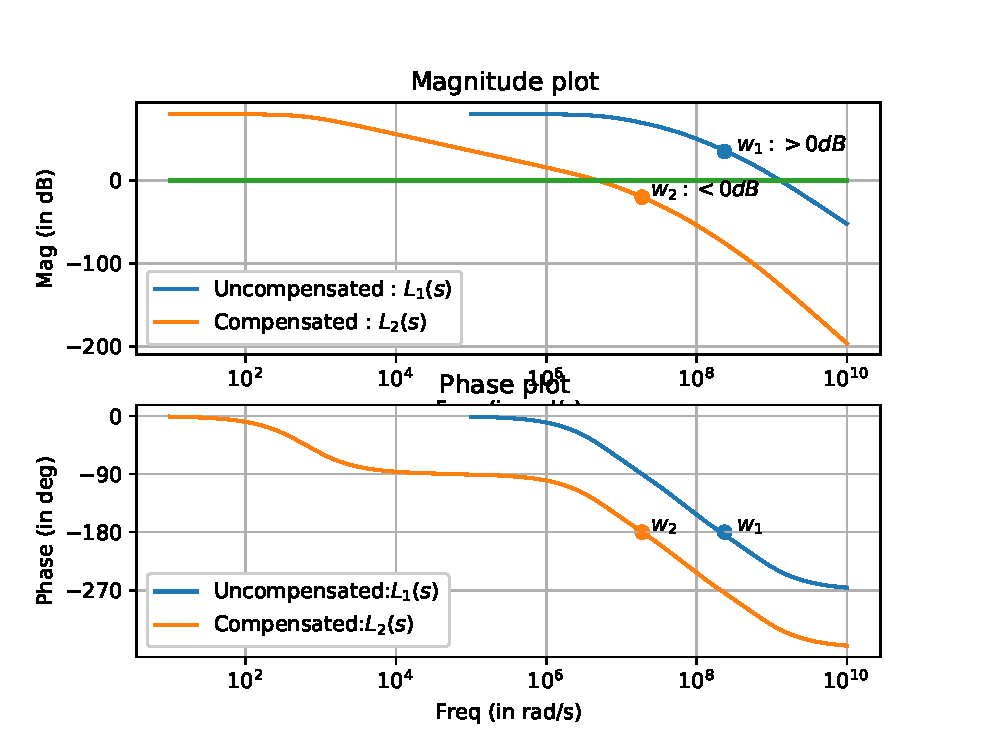
\includegraphics[width=\columnwidth]{./figs/ee18btech11026/ee18btech11026_2.eps}
    \caption{Bode Plots for verificaition}
    \label{fig:ee18btech11026_2}
\end{figure}

From Fig. \ref{fig:ee18btech11026_2},
\begin{align}
\abs{L_1\brak{\j\omega_{180}}} &> 1 
\\
\implies L_{1} &\text{is unstable}
\end{align}
\begin{align}
\abs{L_2\brak{\j\omega_{180}}} & < 1 
\\
\implies L_{2} &\text{is stable}
\end{align}
%
Thus, $H(s)$ stabilizes the unity feedback system.
%Hence the designed Low pass network placed in negative feedback, compensates our open loop gain and stabilizes the closed loop gain of the overall system.
\item Describe the functionality of the feedback circuit.
\\
\solution
The Bode plot of $T(s)$
\begin{figure}[!h]
    \centering
    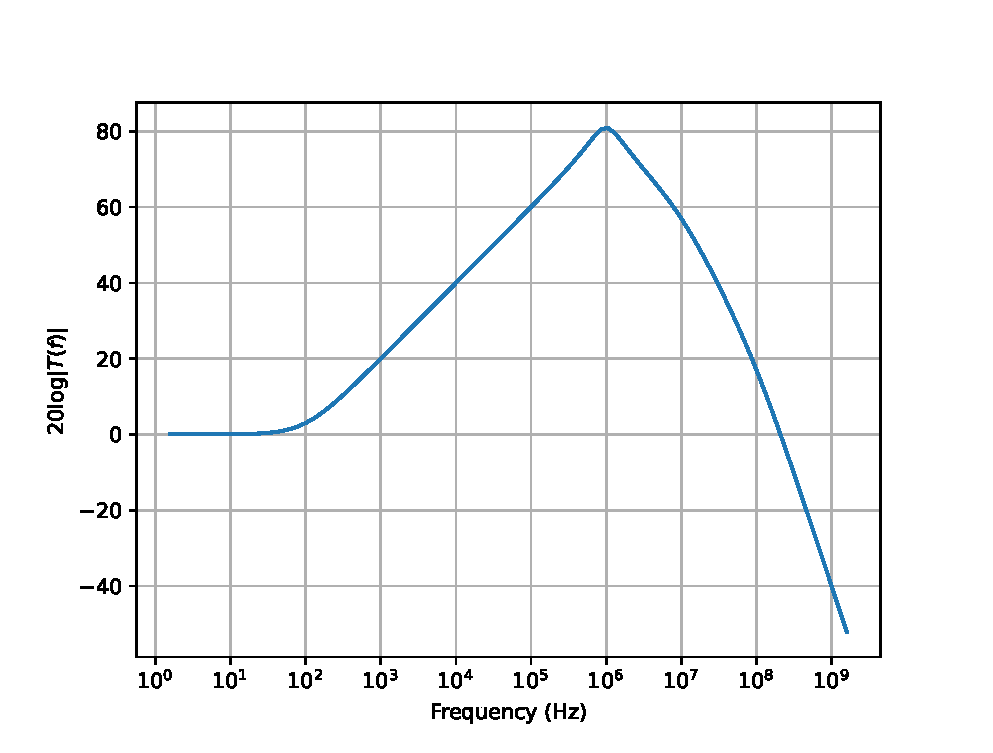
\includegraphics[width=\columnwidth]{./figs/ee18btech11026/Bodeplot.eps}
    \caption{Bode Plots of T(s)}
    \label{fig:ee18btech11026_bode}
\end{figure}
is avaiable in  Fig \ref{fig:ee18btech11026_bode}. This resembles a band pass filter and amplifies the frequencies lying between 0.1 MHz to 10 MHz, while rejecting higher and lower frequencies.
%
\item Simulate the circuit using ngspice.
%\item \textbf{Design a circuit for the given parameters}.\\
%\solution
%
%The below is a block diagram representing G(s) and H(s)
\\
\solution 
The following netlist simulates the unity feedback system. 
\begin{lstlisting}
codes/ee18btech11026/spice/buffer_fb.net
\end{lstlisting}
 The step response in spice is plotted using the following code in Fig. \ref{fig:ee18btech11026_buffer}
 \begin{lstlisting}
codes/ee18btech11026/spice/ee18btech11026_buffer.py
\end{lstlisting}

We can observe that the step response shoots up to a very large value($10^{293}$).This was a consequence for the initial system being unstable.
\begin{figure}[!h]
    \centering
    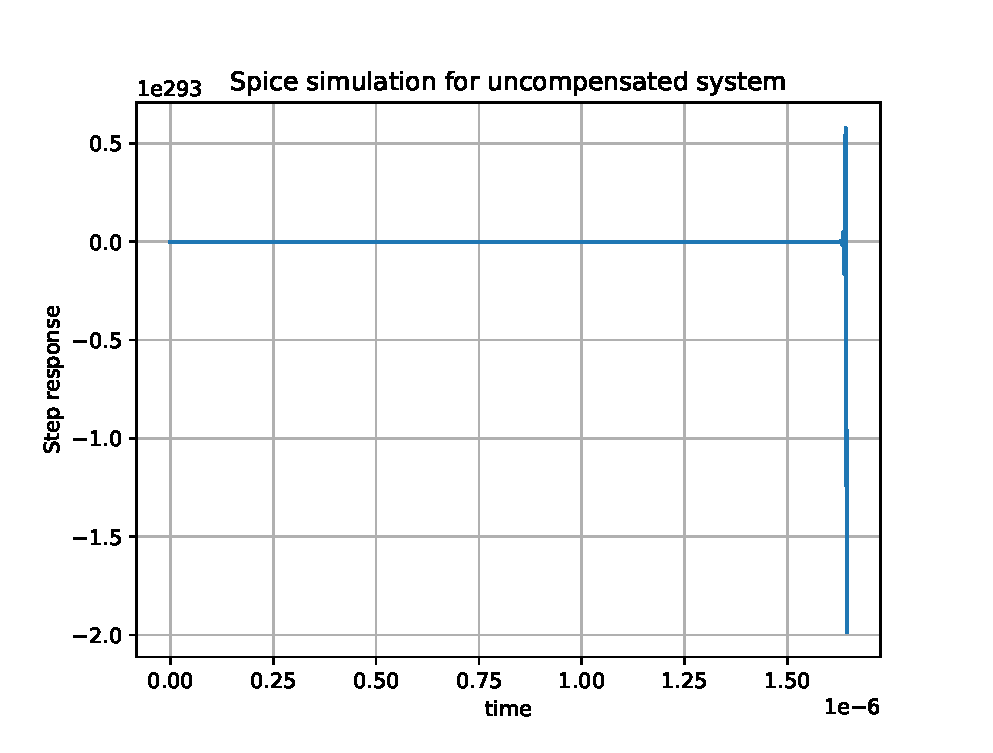
\includegraphics[width=\columnwidth]{./figs/ee18btech11026/ee18btech11026_spice_result_buffer.eps}
    \caption{Step response of Uncompensated System}
    \label{fig:ee18btech11026_buffer}
\end{figure}

The following netlist simulates the compensated system.
   \begin{lstlisting}
codes/ee18btech11026/spice/rc_bf.net
\end{lstlisting}
 The step response in spice is plotted using the following code in Fig. \ref{fig:ee18btech11026_rc_fb}
 \begin{lstlisting}
codes/ee18btech11026/spice/ee18btech11026_rc_fb.py
\end{lstlisting}
Here we can observe that the system has a transient response and it eventually  goes to 1.
\begin{figure}[!h]
    \centering
    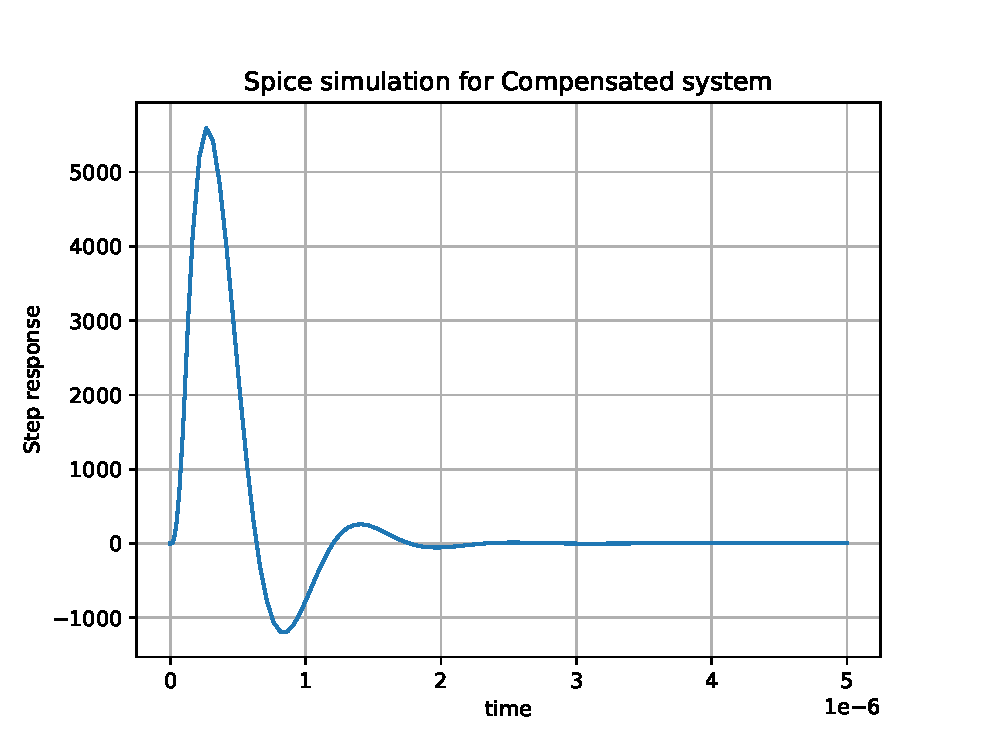
\includegraphics[width=\columnwidth]{./figs/ee18btech11026/ee18btech11026_spice_result_rc_bf.eps}
    \caption{Step response of Compensated System}
    \label{fig:ee18btech11026_rc_fb}
\end{figure}


\begin{figure}[!h]
    \centering
    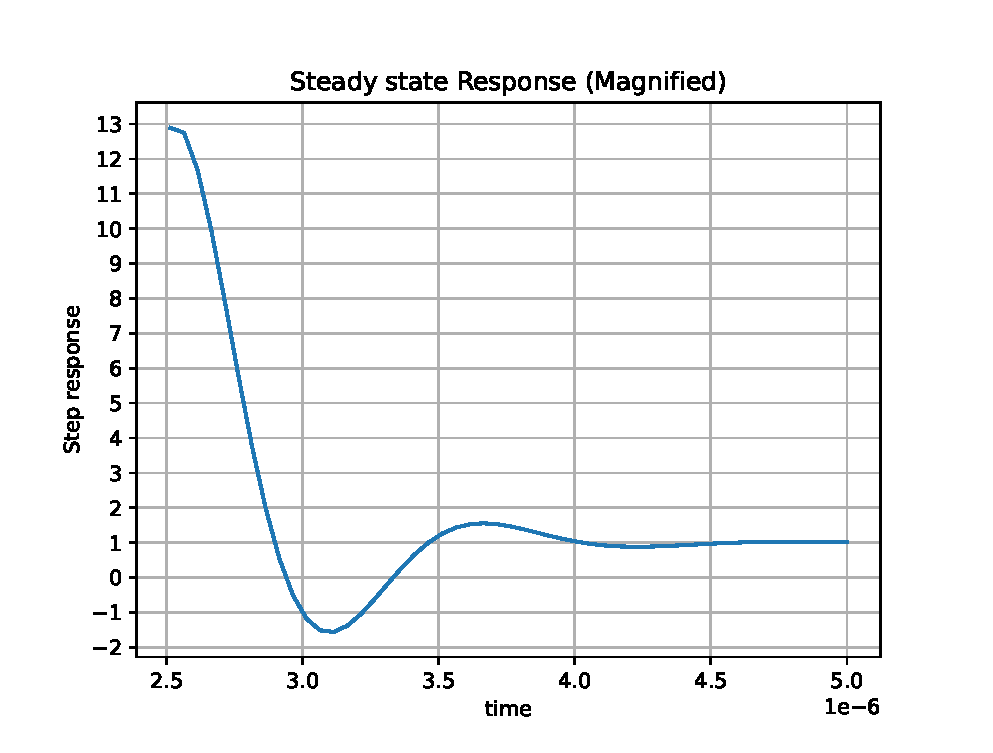
\includegraphics[width=\columnwidth]{./figs/ee18btech11026/ee18btech11026_spice_result_rc_bf_mag.eps}
    \caption{Magnified Plot focussing on steady state}
    \label{fig:ee18btech11026_rc_fb_mag}
\end{figure}


Fig. \ref{fig:ee18btech110026_circuit_2} shows how the circuit is actually implemented in spice using the parameters in Table \ref{table:ee18btech11026_Table_3}  

\begin{figure}[!ht]
	\begin{center}
				\resizebox{\columnwidth}{!}{
\begin{circuitikz}
\ctikzset{bipoles/length=1cm}

\draw 
(-2,1)--(-1,1)--(-1,0) to [R = $RIN$] (-1,0)--(-1,-1)--(-2,-1)


(0, 0) to[I=$ $] (0,0) to (0,-1) %node[ground]{}
(0,0) -- (0,1)--(0.25,1) to[] (1,1) 
to [R = $R_{1}$] (1,-1) 
(1,1)--(2,1)to [C = $C1$](2,-1)
(3,-1)--(3,-1.5)node[ground]{}

(4,0)to [I=$ $] (4,0) to (4,-1)
(4,0) -- (4,1)--(4.25,1) to[] (5,1)
to [R = $R_{2}$] (5,-1) 
(5,1)--(6,1)to [C = $C2$](6,-1)


(8, 0) to[I=$ $] (8,0) to (8,-1) %node[ground]{}
(8,0) -- (8,1)--(8.25,1) to[] (9,1) 
to [R = $R_{3}$] (9,-1) 
(9,1)--(10,1)to [C = $C3$](10,-1)
(0,-1)--(10,-1)

(10,-1)--(12,-1)--(12,0) --(12,1)--(12.5,1)to [R = $Rout$](14,1)

node at(-2,1.25){$V_{+}$}
node at(-2,-1.25){$V_{-}$}
node at(14,1.25){$V_{out}$}
node at(-0.25,0.65){$G1$}
node at(3.75,0.65){$G2$}
node at(7.75,0.65){$G3$}

node at(1,-1.5){$P_{1},GAIN $}
node at(5,-1.5){$P_{2} $}
node at(9,-1.5){$P_{3}$}
;\end{circuitikz}

}
	\end{center}
\caption{Circuit resembling G(s)}
\label{fig:ee18btech110026_circuit_2}
\end{figure}

\begin{table}[!ht]
\centering


%%  This section checks if we are begin input into another file or  %%
%%  the file will be compiled alone. First use a macro taken from   %%
%%  the TeXbook ex 7.7 (suggestion of Han-Wen Nienhuys).            %%
\def\ifundefined#1{\expandafter\ifx\csname#1\endcsname\relax}


%%  Check for the \def token for inputed files. If it is not        %%
%%  defined, the file will be processed as a standalone and the     %%
%%  preamble will be used.                                          %%
\ifundefined{inputGnumericTable}

%%  We must be able to close or not the document at the end.        %%
	\def\gnumericTableEnd{\end{document}}


%%%%%%%%%%%%%%%%%%%%%%%%%%%%%%%%%%%%%%%%%%%%%%%%%%%%%%%%%%%%%%%%%%%%%%
%%                                                                  %%
%%  This is the PREAMBLE. Change these values to get the right      %%
%%  paper size and other niceties.                                  %%
%%                                                                  %%
%%%%%%%%%%%%%%%%%%%%%%%%%%%%%%%%%%%%%%%%%%%%%%%%%%%%%%%%%%%%%%%%%%%%%%

	\documentclass[12pt%
			  %,landscape%
                    ]{report}
       \usepackage[latin1]{inputenc}
       \usepackage{fullpage}
       \usepackage{color}
       \usepackage{array}
       \usepackage{longtable}
       \usepackage{calc}
       \usepackage{multirow}
       \usepackage{hhline}
       \usepackage{ifthen}
%%  End of the preamble for the standalone. The next section is for %%
%%  documents which are included into other LaTeX2e files.          %%
\else

%%  We are not a stand alone document. For a regular table, we will %%
%%  have no preamble and only define the closing to mean nothing.   %%
    \def\gnumericTableEnd{}

%%  If we want landscape mode in an embedded document, comment out  %%
%%  the line above and uncomment the two below. The table will      %%
%%  begin on a new page and run in landscape mode.                  %%
%       \def\gnumericTableEnd{\end{landscape}}
%       \begin{landscape}


%%  End of the else clause for this file being \input.              %%
\fi

%%%%%%%%%%%%%%%%%%%%%%%%%%%%%%%%%%%%%%%%%%%%%%%%%%%%%%%%%%%%%%%%%%%%%%
%%                                                                  %%
%%  The rest is the gnumeric table, except for the closing          %%
%%  statement. Changes below will alter the table's appearance.     %%
%%                                                                  %%
%%%%%%%%%%%%%%%%%%%%%%%%%%%%%%%%%%%%%%%%%%%%%%%%%%%%%%%%%%%%%%%%%%%%%%

\providecommand{\gnumericmathit}[1]{#1} 
%%  Uncomment the next line if you would like your numbers to be in %%
%%  italics if they are italizised in the gnumeric table.           %%
%\renewcommand{\gnumericmathit}[1]{\mathit{#1}}
\providecommand{\gnumericPB}[1]%
{\let\gnumericTemp=\\#1\let\\=\gnumericTemp\hspace{0pt}}
 \ifundefined{gnumericTableWidthDefined}
        \newlength{\gnumericTableWidth}
        \newlength{\gnumericTableWidthComplete}
        \newlength{\gnumericMultiRowLength}
        \global\def\gnumericTableWidthDefined{}
 \fi
%% The following setting protects this code from babel shorthands.  %%
 \ifthenelse{\isundefined{\languageshorthands}}{}{\languageshorthands{english}}
%%  The default table format retains the relative column widths of  %%
%%  gnumeric. They can easily be changed to c, r or l. In that case %%
%%  you may want to comment out the next line and uncomment the one %%
%%  thereafter                                                      %%
\providecommand\gnumbox{\makebox[0pt]}
%%\providecommand\gnumbox[1][]{\makebox}

%% to adjust positions in multirow situations                       %%
\setlength{\bigstrutjot}{\jot}
\setlength{\extrarowheight}{\doublerulesep}

%%  The \setlongtables command keeps column widths the same across  %%
%%  pages. Simply comment out next line for varying column widths.  %%
\setlongtables

\setlength\gnumericTableWidth{%
	60pt+%
	90pt+%
0pt}
\def\gumericNumCols{2}
\setlength\gnumericTableWidthComplete{\gnumericTableWidth+%
         \tabcolsep*\gumericNumCols*2+\arrayrulewidth*\gumericNumCols}
\ifthenelse{\lengthtest{\gnumericTableWidthComplete > \linewidth}}%
         {\def\gnumericScale{\ratio{\linewidth-%
                        \tabcolsep*\gumericNumCols*2-%
                        \arrayrulewidth*\gumericNumCols}%
{\gnumericTableWidth}}}%
{\def\gnumericScale{1}}

%%%%%%%%%%%%%%%%%%%%%%%%%%%%%%%%%%%%%%%%%%%%%%%%%%%%%%%%%%%%%%%%%%%%%%
%%                                                                  %%
%% The following are the widths of the various columns. We are      %%
%% defining them here because then they are easier to change.       %%
%% Depending on the cell formats we may use them more than once.    %%
%%                                                                  %%
%%%%%%%%%%%%%%%%%%%%%%%%%%%%%%%%%%%%%%%%%%%%%%%%%%%%%%%%%%%%%%%%%%%%%%

\ifthenelse{\isundefined{\gnumericColA}}{\newlength{\gnumericColA}}{}\settowidth{\gnumericColA}{\begin{tabular}{@{}p{60pt*\gnumericScale}@{}}x\end{tabular}}
\ifthenelse{\isundefined{\gnumericColB}}{\newlength{\gnumericColB}}{}\settowidth{\gnumericColB}{\begin{tabular}{@{}p{90pt*\gnumericScale}@{}}x\end{tabular}}
\begin{tabular}[c]{%
	b{\gnumericColA}%
	b{\gnumericColB}%%
	}

%%%%%%%%%%%%%%%%%%%%%%%%%%%%%%%%%%%%%%%%%%%%%%%%%%%%%%%%%%%%%%%%%%%%%%
%%  The longtable options. (Caption, headers... see Goosens, p.124) %%
%	\caption{The Table Caption.}             \\	%
% \hline	% Across the top of the table.
%%  The rest of these options are table rows which are placed on    %%
%%  the first, last or every page. Use \multicolumn if you want.    %%

%%  Header for the first page.                                      %%
%	\multicolumn{3}{c}{The First Header} \\ \hline 
%	\multicolumn{1}{c}{colTag}	%Column 1
%	&\multicolumn{1}{c}{colTag}	%Column 2
%	&\multicolumn{1}{c}{colTag}	\\ \hline %Last column
%	\endfirsthead

%%  The running header definition.                                  %%
%	\hline
%	\multicolumn{3}{l}{\ldots\small\slshape continued} \\ \hline
%	\multicolumn{1}{c}{colTag}	%Column 1
%	&\multicolumn{1}{c}{colTag}	%Column 2
%	&\multicolumn{1}{c}{colTag}	\\ \hline %Last column
%	\endhead

%%  The running footer definition.                                  %%
%	\hline
%	\multicolumn{3}{r}{\small\slshape continued\ldots} \\
%	\endfoot

%%  The ending footer definition.                                   %%
%	\multicolumn{3}{c}{That's all folks} \\ \hline 
%	\endlastfoot
%%%%%%%%%%%%%%%%%%%%%%%%%%%%%%%%%%%%%%%%%%%%%%%%%%%%%%%%%%%%%%%%%%%%%%

\hhline{|-|-}
	 \multicolumn{1}{|p{\gnumericColA}|}%
	{\gnumericPB{\centering}\textbf{Elements}}
	&\multicolumn{1}{p{\gnumericColB}|}%
	{\gnumericPB{\centering}\textbf{Value}}

	
\\


\hhline{|--|}
	 \multicolumn{1}{|p{\gnumericColA}|}%
	{\gnumericPB{\centering}$G_{1}$}
	&\multicolumn{1}{p{\gnumericColB}|}%
	{\gnumericPB{\centering}$10^{-2} (V_{+} - V_{-}) A/V$}

\\


\hhline{|--|}
	 \multicolumn{1}{|p{\gnumericColA}|}%
	{\gnumericPB{\centering}$G_{2}$}
	&\multicolumn{1}{p{\gnumericColB}|}%
	{\gnumericPB{\centering}$10^{-6} A/V$}
\\


\hhline{|--|}
	 \multicolumn{1}{|p{\gnumericColA}|}%
	{\gnumericPB{\centering}$G_{3}$}
	&\multicolumn{1}{p{\gnumericColB}|}%
	{\gnumericPB{\centering}$10^{-6} A/V$}
	
\\





\hhline{|--|}
	 \multicolumn{1}{|p{\gnumericColA}|}%
	{\gnumericPB{\centering}$R_{1}$}
	&\multicolumn{1}{p{\gnumericColB}|}%
	{\gnumericPB{\centering}$1M\Omega$}
	
\\


\hhline{|--|}
	 \multicolumn{1}{|p{\gnumericColA}|}%
	{\gnumericPB{\centering}$R_{2}$}
	&\multicolumn{1}{p{\gnumericColB}|}%
	{\gnumericPB{\centering}$1M\Omega$}
	
\\


\hhline{|--|}
	 \multicolumn{1}{|p{\gnumericColA}|}%
	{\gnumericPB{\centering}$R_{3}$}
	&\multicolumn{1}{p{\gnumericColB}|}%
	{\gnumericPB{\centering}$1M\Omega$}
	
\\



\hhline{|--|}
	 \multicolumn{1}{|p{\gnumericColA}|}%
	{\gnumericPB{\centering}$C_{1}$}
	&\multicolumn{1}{p{\gnumericColB}|}%
	{\gnumericPB{\centering}$0.159pF$}
	
\\


\hhline{|--|}
	 \multicolumn{1}{|p{\gnumericColA}|}%
	{\gnumericPB{\centering}$C_{2}$}
	&\multicolumn{1}{p{\gnumericColB}|}%
	{\gnumericPB{\centering}$0.0159pF$}
	
\\


\hhline{|--|}
	 \multicolumn{1}{|p{\gnumericColA}|}%
	{\gnumericPB{\centering}$C_{3}$}
	&\multicolumn{1}{p{\gnumericColB}|}%
	{\gnumericPB{\centering}$0.00159pF$}
	
\\

\hhline{|--|}
	 \multicolumn{1}{|p{\gnumericColA}|}%
	{\gnumericPB{\centering}$R_{IN}$}
	&\multicolumn{1}{p{\gnumericColB}|}%
	{\gnumericPB{\centering}$1000M\Omega$}
	
\\

\hhline{|--|}
	 \multicolumn{1}{|p{\gnumericColA}|}%
	{\gnumericPB{\centering}$R_{OUT}$}
	&\multicolumn{1}{p{\gnumericColB}|}%
	{\gnumericPB{\centering}$100\Omega$}
	
\\

\hhline{|--|}
	 \multicolumn{1}{|p{\gnumericColA}|}%
	{\gnumericPB{\centering}$R_{f}$}
	&\multicolumn{1}{p{\gnumericColB}|}%
	{\gnumericPB{\centering}$1M\Omega$}
	
\\


\hhline{|--|}
	 \multicolumn{1}{|p{\gnumericColA}|}%
	{\gnumericPB{\centering}$C_{f}$}
	&\multicolumn{1}{p{\gnumericColB}|}%
	{\gnumericPB{\centering}$1.59nF$}
	
\\


\hhline{|--|}
	 \multicolumn{1}{|p{\gnumericColA}|}%
	{\gnumericPB{\centering}$R_{s}$}
	&\multicolumn{1}{p{\gnumericColB}|}%
	{\gnumericPB{\centering}$1M\Omega$}











\\
\hhline{|-|-|}
\end{tabular}

\ifthenelse{\isundefined{\languageshorthands}}{}{\languageshorthands{\languagename}}
\gnumericTableEnd




\caption{}
\label{table:ee18btech11026_Table_3}
\end{table}

\end{enumerate}

